\begin{titlingpage}
  \thispagestyle{empty}
  \calccentering{\unitlength} % forudsat \unitlength ikke bruges til andet
  \begin{adjustwidth*}{\unitlength}{-\unitlength}
    \begin{adjustwidth}{-1cm}{-1cm}
      \centering
      { \setlength{\baselineskip}{24pt}
        {\Huge \stext{Kulstof-12{\kern-0.4em}'{\kern-0.4em}s} \par
          % \textit{for}\par
          \stext{henfaldsproces}
        }\par
        \stext{(The decay process of carbon-12)}
        \par\vspace*{4\onelineskip}
        \par
        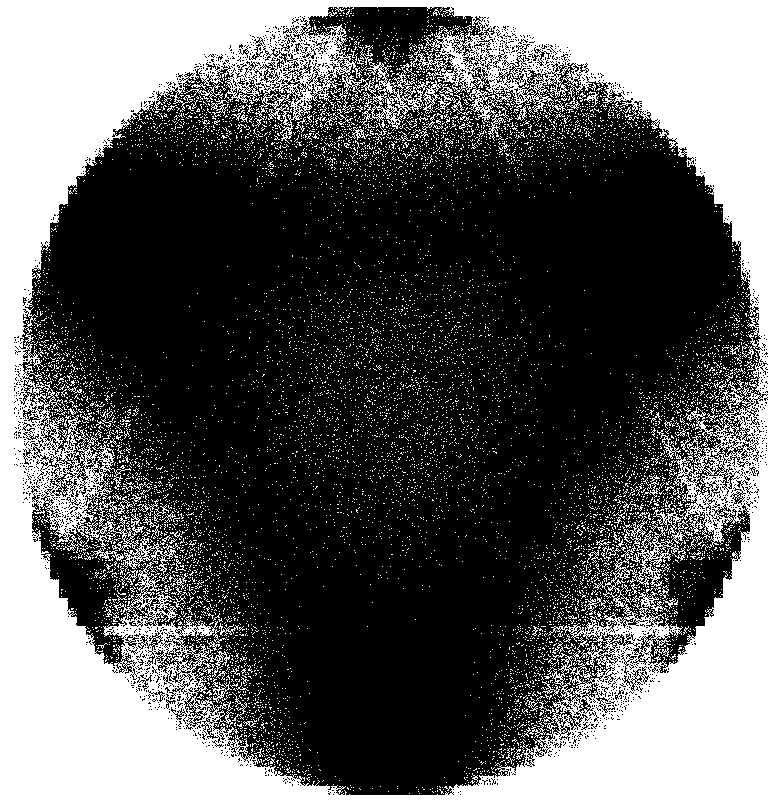
\includegraphics[width=9cm]{forside} 
        \par\vspace*{4\onelineskip}
        \stext{Bachelorprojekt i Fysik}\par
        \large\stext{Michael Kulmback Munch \par 20103561}\par
      }
      \vfill
      \vspace*{2\onelineskip}
      \stext{Vejleder: Hans Fynbo}\hfill
      \stext{26. juni 2013}
      \par\vspace*{2\onelineskip}
      \small
      \stext{Institut for Fysik og Astronomi}\par
      \stext{Aarhus Universitet}
      \enlargethispage{2\onelineskip}
    \end{adjustwidth}
  \end{adjustwidth*}
  % 
  \newpage
  \thispagestyle{empty} % fjerne evt. sidehoved og -fod
  \small
  % resten af teksten indenfor dette env skal være \small
  \strut\vfill  % pres alt ned i bunden af siden
  \begin{flushleft}
    Institut for Fysik og Astronomi \par
    Aarhus Universitet \par
    Ny Munkegade, Bygning 1520 \par
    DK-8000 Aarhus C \par
    Danmark \par
    \vspace{\onelineskip}
    
    \copyright\ Michael Munch 2013 \par
    Version \gitid fra den  \gittime\par
    \vspace{\onelineskip}
    Forsidebilledet er et Dalitzplot af de resulterende $\alpha$-partikler fra henfaldet af exciteret
    tilstand i \Carb produceret ved bestråling af \Bor med 2\MeV protoner.
  \end{flushleft}
\end{titlingpage}